\documentclass{article}
\usepackage{iclr2024_conference,times}

\usepackage[utf8]{inputenc}
\usepackage[T1]{fontenc}
\usepackage[hyphens]{url}
\usepackage{hyperref}
\usepackage{url}
\usepackage{booktabs}
\usepackage{amsfonts}
\usepackage{microtype}
\usepackage{graphicx}
\usepackage{float}
\usepackage{longtable}
\usepackage{tabularx}
\usepackage{caption}
\captionsetup[table]{skip=6pt}

\iclrfinalcopy
\setcitestyle{numbers,square}

\title{How Agent-Ready Is the Web}

\author{Vedang Ratan Vatsa \\
\href{https://veda.ng}{veda.ng}}

\begin{document}
\raggedbottom

\maketitle

\begin{abstract}
AI agents read the same public web that browsers render for people, but agents can fail on pages that people use without friction. JavaScript-only content, missing machine indexes, blocked crawler identities, and absent tool contracts can turn routine agent tasks into errors or inflated token bills. This study measures how often those barriers occur on the public web. The analysis catalogs a 61-check instrument across six layers, builds a deterministic 50,000-domain sample from the Tranco top-1M list with a Chrome User Experience Report overlap flag, and scans each domain with a fixed probe set and a 4,500ms timeout at low concurrency with staggered starts. Reported findings cover all 50,000 domains. Mean readiness score is 25.7 of 100 with a median of 22. Only 6.62\% serve llms.txt, 2.95\% negotiate Markdown, 1.82\% expose a live MCP server, and 54.37\% return non-200 to both tested AI crawler identities, a share that falls to 22.7\% among the 22,855 readable sites. Readiness runs nearly flat across rank tiers rather than concentrating at the top, and one permitting site in five still refuses crawlers at the connection despite its own robots.txt.

\par\medskip
\noindent{\small \textit{Keywords:} AI agents, web measurement, robots.txt, llms.txt, Model Context Protocol, OpenAPI, content negotiation, Tranco, CrUX}

\end{abstract}

\section{Introduction}

An agent that books, cites, or buys over HTTP needs different things from a page than a person with a mouse. People tolerate banners, scripts, and layout. Agents need stable identifiers, plain-text representations, explicit crawler rules, and typed tool contracts. When those are absent, agents must infer structure from layout noise, which risks extra cost and errors.

Section 2 surveys blocking censuses, llms.txt trackers, and a curated commercial board. Each covers one protocol or one selected population. None publishes per-domain probe records for a fixed multi-layer instrument over a stratified random sample. The gap is measurement. Operators lack a baseline for which machine affordances exist, where they cluster by site rank, and which absences cause the most agent failures.

This study addresses that gap with three research questions. First, which machine affordances do public sites publish, by layer and by rank tier. Second, which absences block agents outright as opposed to raising cost. Third, what minimal set of fixes removes the most blocking failures.

The analysis makes four contributions. First, it catalogs a fixed checklist of 61 machine tests, called the instrument below, with exact probes, pass criteria, and the agent failure mode each check guards against. Second, it documents the selection logic for those checks, including exclusions and scoring weights. Third, it builds a seeded 50,000-domain sample from dated public frames with a manifest that records sources, hashes, and tier counts. Fourth, it ships the probe code, sampler, and per-domain records so others can repeat the run.

Section 2 positions the work against related standards and measurement efforts. Section 3 catalogs the instrument. Section 4 records selection and scoring choices. Section 5 describes sampling. Section 6 describes measurement. Section 7 reports results. Section 8 interprets them. Section 9 lists open questions, risks, and limitations. Section 10 closes, with Appendix A tabulating all 61 checks.

\textbf{Data and methodology.} The sampling frame is the Tranco daily top-1M snapshot downloaded on 2026-09-03, with a Chrome User Experience Report (CrUX) global current list from the same week used only as an overlap flag \cite{ref1} \cite{ref2} \cite{ref3}. Tier 1 takes a census of Tranco ranks 1 through 10,000. Tier 2 draws 20,000 uniformly from ranks 10,001 through 100,000. Tier 3 draws 20,000 uniformly from ranks 100,001 through 1,000,000, all under seed 20260903. The observed CrUX overlap in the drawn sample is 23,579 of 50,000. The scanner issues 34 primary HTTP probes plus up to 6 conditional follow-ups per domain, with a 4,500ms per-probe timeout and an identifying User-Agent. Section 6 gives the full probe table and reproduction commands.



\section{Related Work}

Crawler control starts with the Robots Exclusion Protocol, standardized as RFC 9309 \cite{ref4}. That standard tells cooperating crawlers which paths to avoid. It predates answer-engine crawlers such as GPTBot and PerplexityBot, so telling real-time citation bots apart from bulk training scrapers takes per-agent directives. This study tests for that separation directly instead of treating robots.txt as a binary present-or-absent signal.

URL discovery for search crawlers rests on XML sitemaps \cite{ref5}. Sitemaps list canonical URLs but say nothing about agent tools or plain-text mirrors. The llms.txt proposal adds a Markdown index at the domain root for language-model consumers \cite{ref6}. The IETF API catalog proposal standardizes discovery of API entry points and schema locations at a well-known path \cite{ref7}. This study probes all three, because agents use them at different stages of a task.

Execution interfaces come from two families. The Model Context Protocol defines tool and resource access over Streamable HTTP through JSON-RPC, remote procedure calls encoded as JSON \cite{ref8}. Agent-to-agent (A2A) card proposals define peer capability exchange \cite{ref9}. OpenAPI 3.1 defines typed HTTP contracts with schemas and examples \cite{ref10}. OAuth discovery metadata defines how clients find authorization servers and protected resources \cite{ref11} \cite{ref12}. Each specification's standards text describes its own protocol, so combined deployment goes unmeasured. This study checks whether live domains publish them together, since an agent needs the chain, not one link.

Representation negotiation uses HTTP content negotiation, where a client advertises accepted formats and the server selects a representation \cite{ref13}. Link headers advertise related resources such as schemas on any response \cite{ref14}. Rate-limit headers tell clients how to pace requests. These mechanisms decide whether an agent gets clean Markdown or must scrape HTML, which typically costs more tokens to process.

Transport and disclosure standards cover HTTPS enforcement with HSTS \cite{ref15}, content security policy \cite{ref16}, and vulnerability contact files \cite{ref17}. Structured data uses JSON-LD \cite{ref18} and the Schema.org vocabulary for typed entities \cite{ref19}. These predate agents but agents inherit their guarantees, so the instrument includes them as preconditions rather than agent inventions.

Several published measurements cover parts of this ground. The HTTP Archive runs a continuous public crawl of page composition \cite{ref21}. A May 2026 crawl of the Tranco top 10,000 found 5.86\% serving valid llms.txt files and showed raw HTTP 200 counts overstate valid adoption by about 2.7 times, which supports strict pass criteria over status-code counting \cite{ref22}. A June 2026 robots.txt census of the Tranco top 1,000,000 found 63.1\% serving robots.txt with 9.33\% fully blocking at least one major AI crawler \cite{ref23}. An August 2026 census of the Tranco top 100,000 found 19.3\% blocking at least one tracked AI crawler over parseable files \cite{ref24}. A May 2026 survey of the Tranco top 10,000 found 23\% blocking at least one of four major AI bots with sharp category splits \cite{ref25}. Server-log data from 137,000 domains found 97\% of published llms.txt files received zero requests in May 2026, so publication and consumption are separate facts \cite{ref26}. A commercial counterpart takes the opposite sampling path. Ora scores a curated list of agent-relevant companies with 119 behavior-derived checks across four weighted layers, discovery at 20 points through payments at 10, and ranks selected companies rather than sampling the web \cite{ref29}. Curated boards select for operators who already care, while a rank census measures the background rate including everyone who does not. The two designs answer different questions, and the census path differs in three respects. It fixes one instrument across six layers instead of one protocol. It samples by rank tier with a recorded seed instead of hand-picked domains. It stores per-domain probe records instead of aggregate claims alone.



\section{Instrument Catalog}

The scanner evaluates 61 checks in six layers. Each check names its probe, its pass criterion, and the agent failure it guards against. Guarded failures name the risk each check addresses, not a guaranteed outcome on every site. Probe paths below are relative to the domain origin. Two crawler-identity probes replay the homepage fetch under GPTBot and PerplexityBot User-Agents. One negotiation probe replays it under Accept text/markdown.

\subsection{Discovery layer (13 checks)}

Discovery answers whether an agent can find capabilities and boundaries without brute-force crawling. ARD below denotes the Agent Readiness Directory convention used by the scanner host, a single JSON file that points to a domain MCP endpoint, OpenAPI schema, and llms.txt index.

\begin{table}[H]
\centering
\footnotesize
\setlength{\tabcolsep}{4pt}
\sloppy
\begin{tabularx}{\columnwidth}{p{3.2cm}XXX}
\toprule
\textbf{Check} & \textbf{Probe} & \textbf{Pass criterion} & \textbf{Guarded failure} \\
\midrule
robots-ai-policy & GET \url{/robots.txt} & Explicit directives for GPTBot, ClaudeBot, PerplexityBot (partial credit below full) & Accidental exclusion from answers \\
robots-selective-ai-policy & GET \url{/robots.txt} & Separates citation bots from CCBot and ByteSpider & Blanket block removes citations \\
llms-txt & GET \url{/llms.txt}, fallback \url{/.well-known/llms.txt} & Body over 50 chars with Markdown title and links & No curated entry map \\
llms-full & GET \url{/llms-full.txt} or \url{/llms-small.txt} & Body over 100 chars & Multi-hop crawl for full context \\
ard-catalog & GET \url{/.well-known/ard.json} & Parses as JSON & No single agent directory \\
ai-catalog & GET \url{/.well-known/ai-catalog.json} & HTTP 200 with body & AI services undiscoverable \\
api-catalog-rfc9727 & GET \url{/.well-known/api-catalog} & HTTP 200 with body \cite{ref7} & API entry points guessed \\
sitemap-xml & GET \url{/sitemap.xml}, robots-declared or \url{/sitemap_index.xml} fallback & Contains urlset or sitemapindex & New URLs undiscovered \\
sitemap-json & GET \url{/.well-known/sitemap.json} & Body contains JSON object & Parsers pay XML overhead \\
agents-txt & GET \url{/agents.txt} & Body over 20 chars & Action boundaries unknown \\
agents-json & GET \url{/.well-known/agents.json} & HTTP 200 with body & Agent roles unlisted \\
agent-card & GET \url{/.well-known/agent-card.json} & HTTP 200 with body \cite{ref9} & Peer negotiation impossible \\
openai-plugin & GET \url{/.well-known/ai-plugin.json} or \url{/plugin.json} & HTTP 200 with body & Assistant plugin path absent \\
\bottomrule
\end{tabularx}
\end{table}

\subsection{Access layer (9 checks)}

Access answers whether an agent can retrieve readable content at manageable cost. A firewall (WAF) sitting in front of the origin can refuse machine identities while serving browsers, which the bot-identity check below separates from dead hosts.

\begin{table}[H]
\centering
\small
\setlength{\tabcolsep}{4pt}
\sloppy
\begin{tabularx}{\columnwidth}{p{3.2cm}XXX}
\toprule
\textbf{Check} & \textbf{Probe} & \textbf{Pass criterion} & \textbf{Guarded failure} \\
\midrule
markdown-negotiation & GET / with Accept text\url{/markdown} \cite{ref13} & Markdown content type or Markdown body & HTML scrape inflates tokens \\
markdown-twins & GET \url{/index.md} & Body over 50 chars & No static plain-text mirror \\
bot-ua-access & GET / as GPTBot and PerplexityBot & HTTP 200 for both & WAF block on cited sources \\
robots-meta-ai & Homepage meta robots and X-Robots-Tag & Indexable with full-snippet grant & Snippet or index denial \\
link-headers & Homepage Link header \cite{ref14} & describedby, service-desc, or alternate present & Schema undiscoverable per page \\
rate-limit-headers & Homepage rate headers & RateLimit or Retry-After present & Agents trip blind throttles \\
access-js-hydration & Homepage visible text length & Over 300 chars without script execution & Empty page for non-browser agents \\
access-compression & Homepage content encoding & br, zstd, or gzip present & Slow transfers time out \\
access-boilerplate-ratio & Text chars over HTML chars & Ratio at or above 10\% & Tokens spent on boilerplate \\
\bottomrule
\end{tabularx}
\end{table}

\subsection{Usability and MCP layer (10 checks)}

This layer answers whether an agent can act through typed interfaces. Mining-rights metadata follows the TDM Reservation Protocol \cite{ref20}.

\begin{table}[H]
\centering
\small
\setlength{\tabcolsep}{4pt}
\sloppy
\begin{tabularx}{\columnwidth}{p{3.2cm}XXX}
\toprule
\textbf{Check} & \textbf{Probe} & \textbf{Pass criterion} & \textbf{Guarded failure} \\
\midrule
mcp-server-live & POST \url{/.well-known/mcp} and \url{/api/mcp} with initialize \cite{ref8} & JSON-RPC body in reply & No direct tool channel \\
mcp-schema-handshake & Parse of the above reply & capabilities object present & Client cannot negotiate tools \\
openapi-spec & GET \url{/openapi.json}, well-known, or \url{/openapi.yaml} fallback & openapi or swagger marker \cite{ref10} & Endpoints untyped \\
openapi-examples & Parse of the above spec & example fields in parameters & Models invent arguments \\
auth-guide & GET \url{/auth.md} & HTTP 200 with body & Auth path needs a human \\
oauth-agent-discovery & GET \url{/.well-known/oauth-authorization-server} \cite{ref12} & HTTP 200 with body & Token flow undiscoverable \\
tdmrep & GET \url{/.well-known/tdmrep.json} & HTTP 200 with body & Mining rights ambiguous \\
rfc-7807-errors & GET \url{/api} probe & Problem-details shape on errors & Errors unparseable \\
api-dry-run & Header and spec signals & Dry-run or idempotency keys advertised & Agents cannot test safely \\
api-cors-ai & CORS headers on API paths & allow-origin header present & Browser agents blocked \\
\bottomrule
\end{tabularx}
\end{table}

\subsection{Security layer (11 checks)}

Security answers whether agent traffic runs over verified transport with clear disclosure. The HTTPS check verifies the probed origin stayed on https through any redirects. It passes universally by construction of the probe target, so it anchors the security baseline rather than discriminating sites, and no finding in Section 7 leans on it.

\begin{table}[H]
\centering
\small
\setlength{\tabcolsep}{4pt}
\sloppy
\begin{tabularx}{\columnwidth}{p{3.2cm}XXX}
\toprule
\textbf{Check} & \textbf{Probe} & \textbf{Pass criterion} & \textbf{Guarded failure} \\
\midrule
https-tls & Origin scheme & https served & Tampering and downgrade \\
hsts & Strict-Transport-Security header \cite{ref15} & max-age directive present & Protocol downgrade \\
csp & Content-Security-Policy header \cite{ref16} & Header present & Script injection surface \\
xcto & X-Content-Type-Options & nosniff value & MIME-sniffing attacks \\
frame-protection & X-Frame-Options or frame-ancestors & Header or directive present & Clickjacking \\
referrer-policy & Referrer-Policy header & Header present & Leakage of query secrets \\
permissions-policy & Permissions-Policy header & Header present & Unused hardware access \\
security-txt & GET \url{/.well-known/security.txt}, fallback \url{/security.txt} \cite{ref17} & Contact field present & No reporting path \\
security-signatures & GET \url{/.well-known/http-message-signatures-directory} & HTTP 200 with body & Unsigned machine calls \\
security-c2pa & Homepage provenance signals & Manifest or assertion link & Media origin unverifiable \\
security-ai-disclosure & Policy page signals & AI or prompt-injection terms in security or terms files & Model-abuse reports lost \\
\bottomrule
\end{tabularx}
\end{table}

\subsection{SEO and structured data layer (15 checks)}

This layer answers whether answer engines can ground and cite facts. E-E-A-T denotes experience, expertise, authoritativeness, and trust.

\begin{table}[H]
\centering
\small
\setlength{\tabcolsep}{4pt}
\sloppy
\begin{tabularx}{\columnwidth}{p{3.2cm}XXX}
\toprule
\textbf{Check} & \textbf{Probe} & \textbf{Pass criterion} & \textbf{Guarded failure} \\
\midrule
title-tag & Homepage title & Present, unique, under 60 chars & Wrong citation labels \\
meta-description & Homepage meta description & Present, under 160 chars & Missing snippets \\
canonical & Homepage canonical link & Valid canonical URL declared & Index duplication \\
html-lang & html lang attribute & lang attribute present & Wrong language parse \\
favicon-branding & GET \url{/favicon.ico} & File served or icon link declared & No visual citation badge \\
og-tags & Homepage Open Graph tags & title, description, image, url present & Broken previews \\
twitter-cards & Homepage Twitter tags & card and title present & Broken social cards \\
json-ld & Homepage ld+json blocks \cite{ref18} & At least one valid block & No typed facts \\
seo-schema-graph & Parse of ld+json & graph or isPartOf linkage & Disconnected entities \\
seo-rich-schemas & Parse of ld+json & FAQ, Article, or Software types & Thin answer grounding \\
seo-author-eeat & sameAs links & Authoritative profile links & Identity unverifiable \\
seo-answer-first & Heading order & Single h1 before h2 sequence & Poor excerpt selection \\
seo-multimodal & Image alt text & Non-empty alt on content images & Images uncitable \\
seo-freshness & Date metadata & Published or modified dates & Stale answers cited \\
rss-feed & GET \url{/feed.xml} or \url{/feed.json}, head-declared fallback & Valid feed body & No update channel \\
\bottomrule
\end{tabularx}
\end{table}

\subsection{Payments layer (3 checks)}

Payments answers whether agents can settle metered access without a card form.

\begin{table}[H]
\centering
\small
\setlength{\tabcolsep}{4pt}
\sloppy
\begin{tabularx}{\columnwidth}{p{3.2cm}XXX}
\toprule
\textbf{Check} & \textbf{Probe} & \textbf{Pass criterion} & \textbf{Guarded failure} \\
\midrule
agent-payments & Payment headers and homepage markers \cite{ref13} & L402, LSAT, x-payment, x402, or Lightning markers present & No machine billing path \\
payments-webln & WebLN and Lightning signals & Wallet discovery present & No wallet handshake \\
payments-terms & GET \url{/terms-of-use.md} & Machine-readable terms present & Terms need a human reader \\
\bottomrule
\end{tabularx}
\end{table}



\section{Selection Rationale and Scoring}

The 61 checks passed three inclusion tests. First, an agent can test the check with plain HTTP, with no login and no browser. Second, the check maps to a named standard or a documented agent failure, not a taste preference. Third, the probe gives a deterministic pass, warning, fail, or not-applicable verdict that a second run can repeat.

Exclusions follow from the same tests. The instrument skips full browser rendering, login and checkout flows, visual layout scores, and latency percentiles. Those need interactive sessions or repeated timing runs that a one-pass probe cannot support fairly. The paper records them as future work instead of scoring them badly. Five discovery paths (ard.json, ai-catalog.json, agents.txt, agents.json, and agent-card.json) record proposal-stage conventions rather than ratified standards, and the paper treats them as such throughout.

Each check carries a weight of 1 to 3 and an impact tag of critical, important, recommended, or optional. Weights encode the author's severity judgment. Refusing a crawler identity or serving no readable content can block tasks outright and weighs 3, while a missing optional manifest merely closes one discovery path and weighs 1. Grade bands at 95, 85, 70, 55, and 40 are display thresholds, not empirical findings, and the paper never argues from a grade alone. Layer percentages divide earned points by the applicable baseline, with optional checks excluded from the denominator so bonus items cannot drag a conforming site below 100. The 0 to 100 domain score aggregates layer output. Grades map from that score. The code in Section 6 is the normative definition. Prose here describes it. Where prose and code ever disagree, the code release tagged with the run date controls.

The six layers follow an agent task journey in order. Discovery asks whether the agent can find the site, access whether it can read it, usability whether it can act on it, security whether the channel is trustworthy, SEO whether facts can be cited, and payments whether it can settle. Each layer maps to one failure stage, so a low score names the stage where tasks die rather than a vague overall grade. Checks sit in the earliest layer where an agent uses them. A plugin manifest that merely lists an interface belongs to discovery, while the typed OpenAPI contract that executes calls belongs to usability, and mining-rights metadata that governs reuse belongs there for the same reason.

Numeric cutoffs inside checks are published heuristics, not natural constants. The 300-character floor separates empty script shells, which carry near zero visible text, from content pages. The 10\% text-to-HTML ratio separates document pages from application chrome using the same logic. The 50 and 100-character gates reject empty bodies while accepting short manifests. No sensitivity analysis varies these cutoffs, which the limitations record, and every cutoff ships in code so others can test alternatives.

Four instrument settings need explicit defense. The per-probe timeout is 4,500ms, generous against typical response times yet tight enough to bound a 50,000-domain run, and origins slower than that count as unreachable under a cutoff any large-scale agent deployment must impose somewhere. The two replayed crawler identities are GPTBot and PerplexityBot because they span the two bot families of Section 2, bulk training crawlers and citation-driven retrieval bots. ClaudeBot and the rest are parsed in robots.txt but never replayed, so identity-specific conclusions cover only the tested pair. The MCP probe sends initialize and stops there. A successful handshake verdicts exposure without invoking any tool, which keeps the probe non-intrusive. Tool enumeration is left to follow-up work. Probing stays at the homepage and well-known paths because forty requests already strain politeness budgets across 50,000 origins. Deeper per-site crawls belong to site-level follow-ups, not to a census.



\section{Sampling}

The target population is public web hosts that answer HTTP on the standard ports. The list the sample is drawn from, called the sampling frame, is the Tranco daily top-1M snapshot of 2026-09-03.

Tranco is a research ranking, not a vendor leaderboard. Le Pochat and colleagues showed that the major provider lists barely agree with each other, with four combined lists covering 2.82 million sites but agreeing on only around 70,000, so the choice of any single list can severely skew a measurement \cite{ref27}. Tranco answers that problem by averaging provider lists over the previous 30 days with a Dowdall rule, a rank-averaging method that damps daily churn and brief manipulation spikes, and by publishing every daily snapshot under a permanent dated reference that later studies can replay \cite{ref27} \cite{ref28}. Current providers include Cisco Umbrella, Majestic, Farsight, the Chrome User Experience Report, and Cloudflare Radar \cite{ref28}. This study chose Tranco over any single-provider list for three reasons. Dated snapshots make the frame replayable. Thirty-day averaging keeps the head stable across the scan week \cite{ref27}. And hardened aggregation avoids betting the sample on one vendor panel. The Umbrella component carries a known consequence. Umbrella ranks DNS traffic including infrastructure names, so API endpoints, CDN hosts, and DNS names appear in the frame alongside document sites \cite{ref28}. Those hosts legitimately serve nothing agent-readable at their roots, and Section 7 separates them from genuinely walled sites instead of silently dropping them.

The Chrome User Experience Report supplies real-user field data from Chrome, published monthly as an unranked set of popular destinations \cite{ref2} \cite{ref27}. Because the list is monthly and unranked, its own documenters note it cannot replace a ranking \cite{ref27}. This study therefore uses the CrUX global current list from the same week only as an overlap flag for popularity cross-checks \cite{ref2} \cite{ref3}. CrUX measures Chrome real-user traffic, so the flag carries Chrome's population bias and the paper reads it as popularity signal, not ground truth \cite{ref27}. CrUX never filters the sample. It only labels it.

Tier 1 takes a census of Tranco ranks 1 through 10,000 (10,000 domains). A census counts every member instead of sampling, which removes sampling noise exactly where cited examples come from, and a top-10k census stays directly comparable with the Thunderbit and Crawlmind top-10k studies \cite{ref22} \cite{ref25}. Tier 2 draws 20,000 uniformly from ranks 10,001 through 100,000. Tier 3 draws 20,000 uniformly from ranks 100,001 through 1,000,000. Both draws sample without replacement through a seeded generator. A seed number fixes the random draw, so rerunning with seed 20260903, dated as the draw day, selects the same domains on any machine. Equal mid and tail draws give both groups comparable precision instead of letting the tail drown in its own size. The sample is therefore not the first 50,000 ranks, which would exclude the entire long tail and answer only how popular sites behave. Tiers assume rank orders agent-relevant exposure, an approximation the CrUX split of Section 7.8 tests rather than takes for granted. Sample sizes follow precision math. At 2,000 validation domains the sampling wobble (standard error) runs about 0.5 points on single-digit shares and about 1.1 points near 40\%, which is why the validation claims hold within the bands Section 7 states. The 100-domain concurrency control and the 300-domain re-verification are tripwires sized to detect double-digit systematic shifts in minutes, not estimates in their own right. The low-band re-scan covers scores of 10 and below because stale failures cluster at the score-6 floor with a small margin above it. Outputs are domains.txt for scan order, sample.csv with rank, tier, and CrUX overlap per domain, and manifest.json with source stamps, SHA-256 hashes, seed, tier counts, and the observed overlap of 23,579 of 50,000. The draw replays exactly from the seed and the dated snapshots.



\section{Measurement}

Each domain receives 34 primary probes covering the paths in Section 3, plus up to 6 conditional follow-ups for declared sitemaps, legacy security.txt, well-known llms.txt, OpenAPI YAML, sitemap indexes, and head-declared feeds. Probes address the apex origin exactly as listed, with no www-subdomain fallback, so hosts serving only on www read as absent and the limitations record that boundary. The engine fans probes out in parallel under an AbortController timeout of 4,500ms per probe. Two homepage replays rotate the User-Agent to GPTBot and PerplexityBot. One replay sets Accept to text/markdown. Two MCP probes POST a JSON-RPC initialize payload to the well-known and API paths \cite{ref8}.

Verdicts map to four states. Pass means the artifact exists and meets the criterion. Warning means a partial or unlinked artifact. Fail means absence or a blocking response. Not-applicable covers checks gated on a live dependency, such as handshake validation without a live MCP endpoint. Scores follow Section 4.

The batch runner reads domains.txt, resumes from results.jsonl, and runs a fixed worker pool. The full run uses parallel processes over disjoint domain shards, with per-shard outputs merged and deduplicated by domain afterward. Requests hit each domain origin only, identify the scanner in the User-Agent with a contact URL so operators can allowlist or query the traffic, and cap concurrency so no single host receives parallel bursts beyond the fixed probe set. The run stores only HTTP metadata needed for verdicts. It stores no cookies, submits no forms, and rejects private hostnames and literal private-IP addresses before any probe runs. A progress log records counts and elapsed time.

Validation rests on three legs. A 2,000-domain validation run under gentle settings completed first with zero transport failures and predicted final headline shares within six points. Pacing was set by calibration, not by guess. An early high-concurrency pass returned a 95.4\% homepage-failure rate, while the same population under gentle settings measured 61.5\%, three re-scanned sites rose from scores of 6 to between 37 and 46, and a concurrency-1 control measured 56.8\%. The hurried pass was therefore discarded and the corpus re-scanned gently. Layer percentages recompute from the stored per-check map, so a scoring bug shows as a mismatch instead of hiding in prose. Every number in Section 7 traces to a released per-domain row, and row counts accompany each table.



\section{Results}

\subsection{Response and coverage (N=50,000)}

The reported corpus scanned all 50,000 sample domains three at a time with starts seconds apart, under a watchdog loop, a supervisor that relaunched dead workers with resume. Workers died silently several times overnight, likely memory pressure, and resume kept every completed row. All 50,000 domains returned scored rows with zero missing. A seeded 2,000-domain validation subset scanned first under the same regime predicted the final mean within three points and every headline share within six points, which the text notes where the comparison matters. A low-band re-scan of the lowest-scoring domains then refreshed conservative shares by latest verdict, as Limitations describes.

\begin{table}[H]
\centering
\small
\setlength{\tabcolsep}{4pt}
\sloppy
\begin{tabular}{ll}
\toprule
\textbf{Outcome} & \textbf{Reported corpus (N=50,000)} \\
\midrule
Attempted & 50,000 \\
Completed with HTTP verdicts & 50,000 \\
DNS or transport failures & 0 missing \\
Homepage readable without script execution & 45.71\% \\
Mean score, 0 to 100 & 25.7 \\
\bottomrule
\end{tabular}
\end{table}

\subsection{Adoption by check (N=50,000)}

The eleven headline checks span all six layers, one leading indicator per layer focus with extra seats for crawler reachability and execution interfaces. At N=50,000 the 95\% intervals run about ±0.2 points on single-digit shares and ±0.4 points near 40\%, so reported differences of whole points stand clear of sampling noise. Pass shares below count full and partial-credit passes. The robots-ai-policy check grants partial credit for covering some but not all tested crawler identities, so its pass share overstates strict full-policy adoption and the text says so where it matters. The validation subset predicted each of these shares within six points, with llms-txt at 6.75\% against 5.70\% final.

\begin{table}[H]
\centering
\small
\setlength{\tabcolsep}{4pt}
\sloppy
\begin{tabularx}{\columnwidth}{p{3.2cm}XXX}
\toprule
\textbf{Layer} & \textbf{Check} & \textbf{Pass count} & \textbf{Pass share} \\
\midrule
Discovery & robots-ai-policy & 21,881 & 43.76\% \\
Discovery & llms-txt & 3,310 & 6.62\% \\
Access & markdown-negotiation & 1,474 & 2.95\% \\
Access & bot-ua-access & 18,912 & 37.82\% \\
Usability & mcp-server-live & 910 & 1.82\% \\
Usability & openapi-spec & 78 & 0.16\% \\
Security & https-tls & 50,000 & 100.00\% \\
Security & security-txt & 2,288 & 4.58\% \\
SEO & json-ld & 10,687 & 21.37\% \\
SEO & seo-author-eeat & 6,910 & 13.82\% \\
Payments & agent-payments & 163 & 0.33\% \\
\bottomrule
\end{tabularx}
\end{table}

The bot-identity split needs separate reporting. Both tested crawler identities received HTTP 200 success responses on 18,912 domains (37.82\%). Exactly one of the two succeeded on 3,901 domains (7.80\%). Both failed on 27,187 domains (54.37\%). That last share mixes dead hosts with walled ones, so the paper decomposes it below. Appendix A tabulates all 61 checks.

Restricting to the 22,855 readable domains, those passing the hydration check, changes the numbers. Both identities succeed on 15,080 (65.98\%), one succeeds on 2,578 (11.28\%), and both fail on 5,197 (22.74\%). Conditional adoption on readable sites runs higher across the board. Robots-ai-policy passes on 70.89\%, llms-txt on 12.50\%, markdown-negotiation on 6.35\%, MCP on 3.89\%, sitemaps on 50.12\%, and JSON-LD on 45.71\%, with a conditional mean score of 41.1. The gap between unconditional and conditional shares measures how much of the unreadiness problem is reachability rather than missing standards.

\begin{figure}[H]
\centering
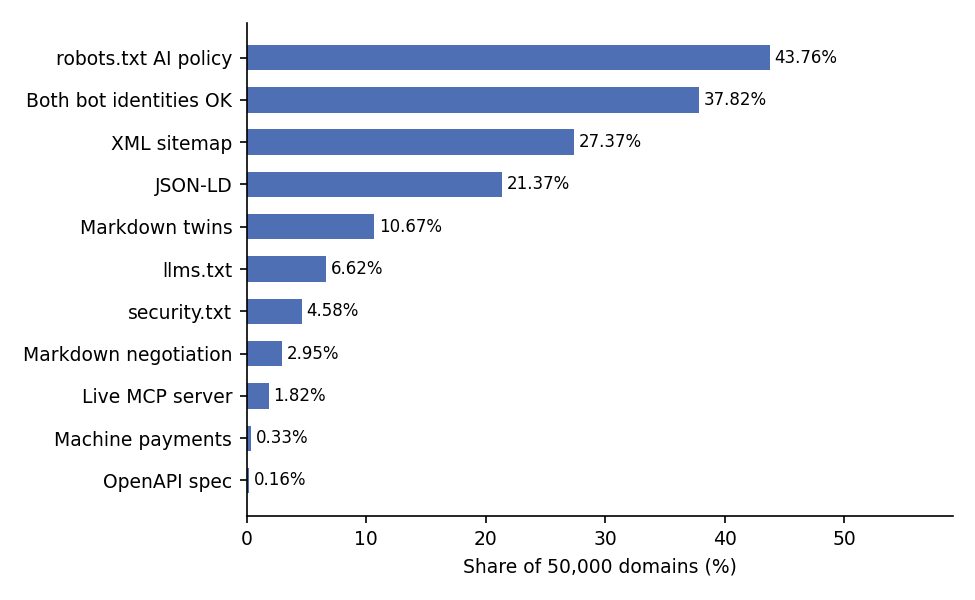
\includegraphics[width=0.9\columnwidth]{figures/fig1_adoption.png}
\caption{Pass shares for eleven headline checks across all 50,000 domains, sorted ascending.}
\end{figure}

\subsection{Scores by rank tier (N=50,000)}

\begin{table}[H]
\centering
\small
\setlength{\tabcolsep}{4pt}
\sloppy
\begin{tabularx}{\columnwidth}{p{3.2cm}XXXX}
\toprule
\textbf{Tier} & \textbf{N} & \textbf{Mean 0 to 100} & \textbf{Median} & \textbf{Share refused on both bot identities} \\
\midrule
Tier 1 (ranks 1-10k) & 10,000 & 26.1 & 23 & 56.2\% \\
Tier 2 (ranks 10k-100k) & 20,000 & 25.2 & 20 & 55.6\% \\
Tier 3 (ranks 100k-1M) & 20,000 & 25.9 & 22 & 52.2\% \\
\bottomrule
\end{tabularx}
\end{table}

Grade distribution across the 50,000 domains is A on 4, B on 496, C on 3,616, D on 9,740, and F on 36,144. Tier means sit within one point of each other, so prominence buys no readiness advantage. Only refusal rates keep a clear direction, falling toward the tail. The pre-registered top-heavy reading is refuted in Section 8.

\begin{figure}[H]
\centering
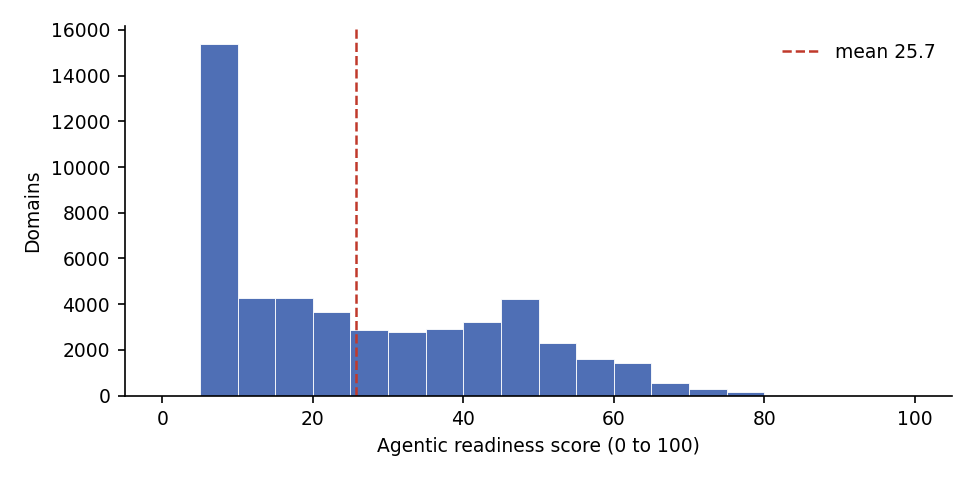
\includegraphics[width=0.9\columnwidth]{figures/fig2_score_hist.png}
\caption{Distribution of 0 to 100 readiness scores across all 50,000 domains with the mean marked.}
\end{figure}

\begin{figure}[H]
\centering
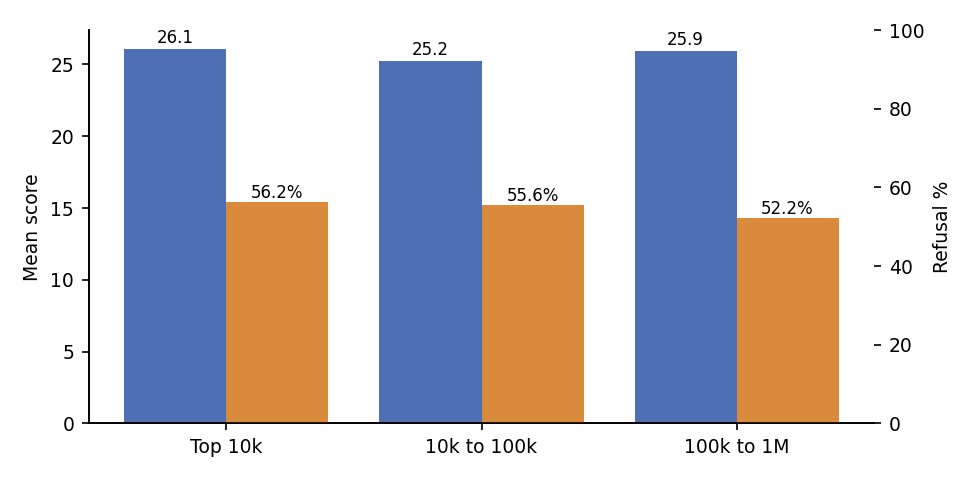
\includegraphics[width=0.9\columnwidth]{figures/fig3_tier_compare.png}
\caption{Mean score and both-identity refusal share by rank tier.}
\end{figure}

Plausible drivers of the flat means alongside falling refusal rates are the concentration of API endpoints, CDN hosts, and aggressive WAF defaults at the top of the ranking against plainer document sites in the long tail. The pre-registered top-heavy reading is refuted in Section 8.

\begin{figure}[H]
\centering
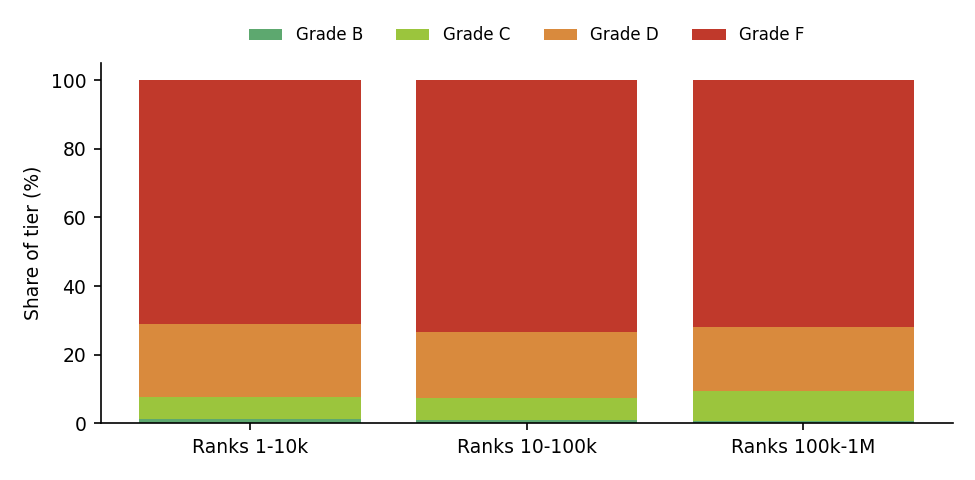
\includegraphics[width=0.9\columnwidth]{figures/fig4_grades_by_tier.png}
\caption{Grade mix by rank tier. Four A grades are too small to display.}
\end{figure}

\subsection{MCP follow-up}

Manual re-probing of a sample of the 910 MCP-pass domains with an independent HTTPS client showed byte-identical initialize responses across unrelated stores, with a tools list exposing a catalog-search tool that identifies itself as Shopify-hosted. The verdicts are genuine live servers, but the adoption they record is platform-default exposure rather than per-operator deployment. The paper reports exposure and labels it as such. The protocol's capability-negotiation step (handshake) passes strictly on only 3 of the 910, but that gap is a parser limitation worth stating plainly. The engine parses the first non-empty reply body as JSON, which fails on error pages and framed transports even when the sibling endpoint holds valid JSON, so the handshake column understates negotiation and the exposure column carries the finding.

\subsection{Layer profile}

Mean layer scores across all 50,000 domains run highest on security at 41.0 and lowest on usability at 7.4, with discovery at 20.7, access at 23.9, SEO at 28.9, and payments at 9.8. The ordering is the finding. Transport hardening from the human web appears to transfer to agents for free, while anything invented for agents specifically sits near zero. Across tiers the layer pattern is mixed rather than uniform. Access and usability rise toward the tail, security falls toward the tail consistent with enterprise hardening concentrated at the head, and discovery, SEO, and payments stay roughly flat. No single tier leads everywhere, which matches the flat overall means of Section 7.3.

\begin{figure}[H]
\centering
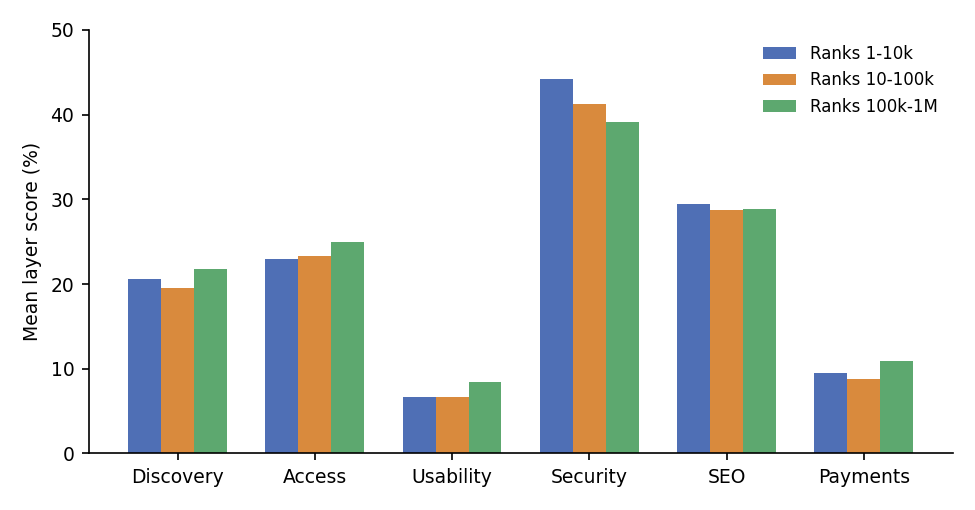
\includegraphics[width=0.9\columnwidth]{figures/fig5_layers_by_tier.png}
\caption{Mean layer scores by rank tier.}
\end{figure}

\subsection{Failure concentration}

The third research question asks for the minimal fix set, and the data refuses one. Counting every fail and partial verdict as one failure instance yields 2,145,053 instances across the corpus, and the fifteen most-failed checks together cover only 33.5\% of them. Fifteen rows keep the chart readable while the appendix carries all 61. Unreadiness is broad-spectrum. No three-file or five-header remedy moves the mean far, because the long tail of misses stretches across all 61 checks. The practical reading points back to platforms. Defaults shipped by frameworks, commerce platforms, and CDNs are the best-placed lever to move dozens of checks at once, which is also the only adoption mechanism observed working at scale in Section 7.4.

\begin{figure}[H]
\centering
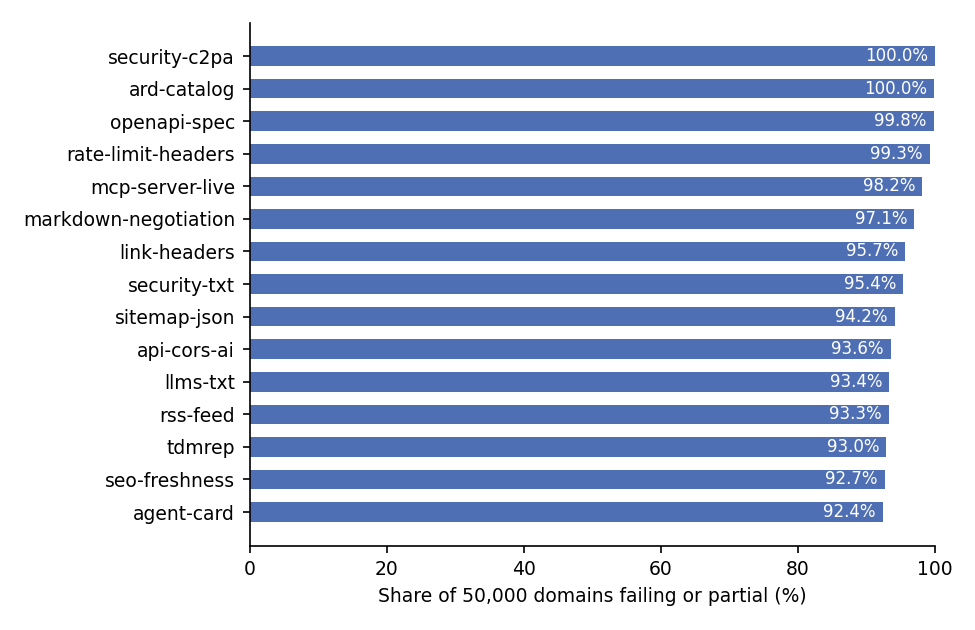
\includegraphics[width=0.9\columnwidth]{figures/fig6_failure_pareto.png}
\caption{The fifteen most-failed checks by share of domains, counting fail and partial verdicts.}
\end{figure}

\subsection{Policy versus behavior}

Robots.txt states policy and servers enforce behavior, and the two disagree in both directions. Among the 21,881 domains whose robots.txt passes the AI-policy check, 14,706 serve both crawler identities (67.2\%), 2,556 serve one (11.7\%), and 4,619 refuse both (21.1\%). One site in five that permits AI crawlers on paper still refuses them at the connection. The reverse gap is smaller but real. Among 24,481 domains with no AI-bot policy at all, 3,173 (13.0\%) serve both identities anyway. Selective policies sit in between and lean restrictive. Of 3,638 partially covered domains, 2,393 (65.8\%) refuse both identities, consistent with operators who write granular rules in order to block.

\begin{figure}[H]
\centering
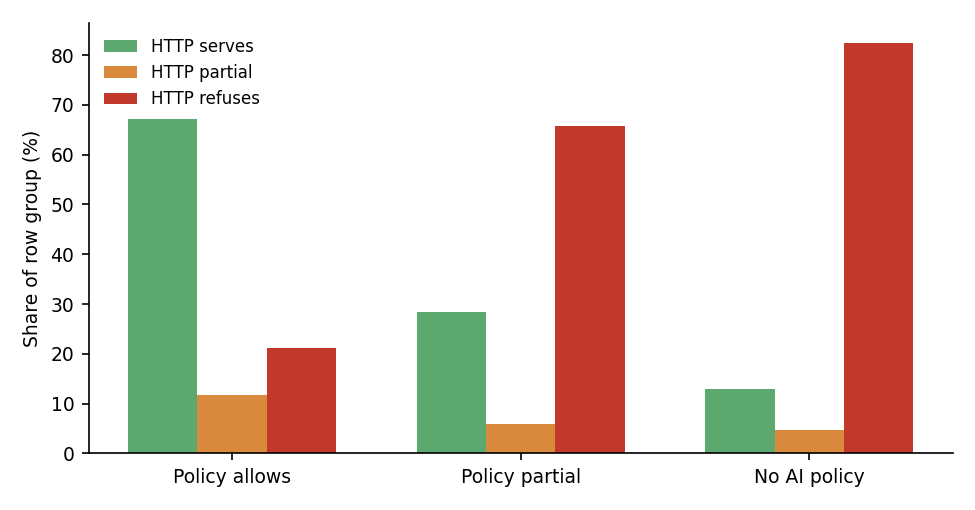
\includegraphics[width=0.9\columnwidth]{figures/fig7_policy_behavior.png}
\caption{HTTP behavior toward crawler identities grouped by robots.txt policy verdict.}
\end{figure}

\subsection{Popularity split}

CrUX-listed domains adopt at roughly twice the rate of unlisted ones on every headline check. llms-txt passes on 8.87\% of the 23,579 listed domains against 4.61\% of the 26,421 unlisted ones. MCP exposure runs 2.83\% against 0.92\%. Both bot identities succeed on 45.77\% against 30.74\%. Markdown negotiation reaches 4.02\% against 1.99\%. Explicit AI-bot policy stands at 54.56\% against 34.12\%. Popularity predicts readiness better than rank tier does. Tier means move only about three points while the CrUX split roughly doubles every headline share, which refines the inversion of Section 7.3.

An external cross-check supports the instrument. Twenty-five domains on this census also appear on Ora's curated agent-readiness board \cite{ref29}, and they average 65.8 on this instrument against the 25.7 background, with the highest-traffic developer platforms at the top of both orderings. The instruments differ too much for score-to-score comparison, but agent-forward companies landing far above background on both is the convergent signal a new instrument needs.



\section{Discussion}

The pre-registered plan named three patterns and tied each to a remedy. The final data selects among them, and overrules one.

The top-heavy pattern does not appear. Tier means sit within one point of each other while refusal rates fall toward the tail, so prominence buys no readiness advantage. Plausible drivers are infrastructure endpoints and strict WAF defaults concentrated at the top of the ranking. That outcome favors hosted defaults from frameworks and platforms over outreach pitched at large sites. The MCP follow-up supports the same reading. The clearest adoption signal in the corpus arrives as a platform default, not as thousands of independent operator decisions.

The blocking-heavy pattern appears clearly. Both tested crawler identities fail on 54.37\% of domains, and on 22.74\% of readable ones, while transport checks pass universally, which may indicate that security defaults rather than missing standards cause most agent failures. That outcome favors allow-list guidance for verified crawler identities over new spec work.

The cost-heavy pattern appears alongside it. Markdown negotiation passes on 2.95\% of domains while basic encrypted delivery (HTTPS) passes universally, which may indicate that agents pay a token tax on almost every read. That outcome favors server-side Markdown rendering as a cheap near-term fix per unit of agent cost removed.

Each reading ties to a different remedy. Distribution gaps call for hosted defaults from frameworks and CDNs. Blocking gaps call for documented WAF exceptions. Cost gaps call for representation fixes. The completed Section 7 decides among them, and it selects all three remedies with platform defaults first.

Outcomes by research question follow directly. First, published affordances concentrate in inherited transport and metadata. Security averages 41.0 and JSON-LD passes on 21.37\%, while agent-native checks sit near zero with MCP at 1.82\% and Markdown negotiation at 2.95\%. Second, outright blocks dominate added cost as the failure mode. Over half of bot-identity refusals come from unreachable or refusing origins rather than heavy pages, and readable sites still refuse both crawler identities at 22.74\%. Third, no minimal fix set exists, with the top fifteen misses covering about one third of failure instances.

Seven learnings stand out. One, unreadiness splits roughly half and half between reachability and missing standards, since conditional shares on readable sites run roughly double the unconditional ones. Two, prominence does not buy readiness. No tier leads everywhere, and the head leads only security while trailing the tail on access and usability. Three, adoption arrives through platforms more visibly than through persuasion. The only large-scale MCP presence in the corpus is a commerce default at 1.82\%, while payment rails sit under half a percent and proposal-stage directories without a platform behind them stay under eight. Four, the cheapest win needs no new standard. One permitting site in five refuses crawlers at the connection, and aligning policy files with firewall behavior is configuration work. Five, popularity predicts twice the adoption of obscurity on every headline check, so platform defaults aimed at trafficked sites propagate furthest. Six, publication is not consumption. Most machine artifacts this study counts have unknown readership, and the llms.txt server-log literature finds nearly all files unread. Seven, measurement at this scale needs pacing calibration. Fetch verdicts from an overloaded source network describe that network, and this study discarded its first full pass after proving exactly that.

Two later analyses sharpen the prescription. The failure concentration of Section 7.6 answers the third research question directly. No minimal fix set exists at the operator level, because misses spread across all 61 checks with the top fifteen covering under one third of instances. The consistency analysis of Section 7.7 locates a cheap coordination win available. One site in five already permits AI crawlers in robots.txt and refuses them over HTTP, a misalignment no new standard needs to fix. Server templates that align the two, plus documented WAF exceptions for verified crawler identities, can remove the most tractable large block without asking operators to learn anything new. The popularity split of Section 7.8 orders the outreach. Traffic-measured popular sites adopt at twice the rate of the rest, so defaults shipped through the platforms serving those sites can propagate furthest per integration.



\section{Open Questions and Risks}

Standards maturity stays uneven. The llms.txt format is a proposal with real adoption but no RFC number \cite{ref6}. Agent directories themselves are fragmented. The instrument probes four competing formats, agents.json manifests, ARD catalogs, A2A agent cards, and plugin manifests, because no single declaration won \cite{ref9}. Payment headers for agents lack one settled path. Operators who adopt early may need to support parallel formats for a period.

A public readiness score can guide bulk scrapers as well as defenders. The paper separates citation bots from training scrapers in the robots checks for this reason \cite{ref4}, and the scanner identifies itself on every probe. Operators can reproduce any verdict from the probe table and then decide their own crawling policy.

\subsection{Limitations}

The run observes homepages and well-known paths from one network vantage point across a nineteen-hour window spanning September 3 to 4, 2026. It does not render JavaScript, follow login flows, or test interactive checkouts. It does not measure latency distributions. Probes address apex origins with no www fallback, so www-only hosts read as absent. The snapshot is single, so the paper makes no trend claims about adoption rising or falling. Single-pass rows can freeze transient failures, and a 300-domain re-verification sample found 41 rows rising twenty or more points on re-scan against zero falling that far. A full low-band re-scan of all 21,247 sub-11 scores then refreshed the corpus by latest verdict, which is the version this paper reports. WAF behavior can vary by source network, so bot-identity verdicts describe the scanner vantage point and may differ elsewhere. Sector labels are absent by design, since the sample stratifies by rank tier with a recorded seed rather than by hand-built sector lists. A single mean across tiers can hide tier differences, so Section 7 reports tiers separately.



\section{Conclusion}

The web is not ready for its machine visitors. Across 50,000 domains the mean readiness score is 25.7, the median is 22, and more than seven in ten domains fail outright. The failures have a shape. Reachability causes about half, missing agent standards cause the rest, prominence buys no advantage across tiers, popularity predicts plenty, and the only fixes observed working at scale arrive as platform defaults rather than operator decisions.

What changes this picture is coordination more than invention. The largest tractable wins need no new protocol. Aligning robots.txt policy with firewall behavior, serving Markdown alongside HTML, and shipping machine manifests as framework defaults would move every layer this study measures.

These numbers describe the sampled host population, and the sample's shape explains them. Because the Tranco frame ranks DNS traffic rather than document sites, API endpoints, CDN hosts, and infrastructure names fill part of every tier and legitimately serve nothing agent-readable, which is why more than half of origins read as unreachable before any standard is evaluated. Because the strata run 10,000, 20,000, and 20,000 rather than traffic-weighted, the 25.7 mean counts an obscure tail host equally with a top-100 site. To the extent agent traffic follows user traffic toward popular destinations, where this study measures roughly double the adoption, per-visit readiness runs better than the per-host mean suggests. The operator-relevant reading is therefore the conditional one. Among readable sites the mean is 41.1, sitemaps pass on half, and two crawler identities succeed on two thirds. A low-band re-scan already lifted the conservative early shares once, and repeated snapshots over time would show whether defaults are spreading or stalling. Until then, any agent venturing onto the public web should expect most doors to be unmarked, many locked, and a few wide open.



\section*{Appendix A. Full 61-check verdict counts (N=50,000)}

Partial covers warning verdicts including partial-credit passes. Gated covers not-applicable verdicts on checks that need a live dependency. Three criteria read permissively by design and their pass counts are upper bounds. Robots-meta-ai passes any page without an explicit noindex or nosnippet signal, seo-multimodal passes pages with no images at all, and security-ai-disclosure matches keyword substrings rather than verified policy text.

\begin{center}
\footnotesize
\setlength{\tabcolsep}{3pt}
\begin{longtable}{p{2.6cm}lllll}
\toprule
\textbf{Layer} & \textbf{Check} & \textbf{Pass} & \textbf{Partial} & \textbf{Fail} & \textbf{Gated} \\
\midrule
Discovery & robots-ai-policy & 21881 & 3638 & 24481 & 0 \\
Discovery & robots-selective-ai-policy & 4420 & 21099 & 24481 & 0 \\
Discovery & llms-txt & 3310 & 5418 & 41272 & 0 \\
Discovery & llms-full & 5771 & 44229 & 0 & 0 \\
Discovery & ard-catalog & 20 & 3566 & 46414 & 0 \\
Discovery & ai-catalog & 3890 & 46110 & 0 & 0 \\
Discovery & api-catalog-rfc9727 & 3883 & 46117 & 0 & 0 \\
Discovery & sitemap-xml & 13686 & 3581 & 32733 & 0 \\
Discovery & sitemap-json & 2903 & 47097 & 0 & 0 \\
Discovery & agents-txt & 4136 & 45864 & 0 & 0 \\
Discovery & agents-json & 3828 & 46172 & 0 & 0 \\
Discovery & agent-card & 3791 & 46209 & 0 & 0 \\
Discovery & openai-plugin & 4817 & 45183 & 0 & 0 \\
Access & markdown-negotiation & 1474 & 0 & 48526 & 0 \\
Access & markdown-twins & 5337 & 44663 & 0 & 0 \\
Access & bot-ua-access & 18912 & 3901 & 27187 & 0 \\
Access & robots-meta-ai & 46390 & 0 & 3610 & 0 \\
Access & link-headers & 2173 & 47827 & 0 & 0 \\
Access & rate-limit-headers & 361 & 49639 & 0 & 0 \\
Access & access-js-hydration & 22855 & 0 & 27145 & 0 \\
Access & access-compression & 28210 & 21790 & 0 & 0 \\
Access & access-boilerplate-ratio & 7737 & 42263 & 0 & 0 \\
Usability & mcp-server-live & 910 & 49090 & 0 & 0 \\
Usability & mcp-schema-handshake & 3 & 907 & 0 & 49090 \\
Usability & openapi-spec & 78 & 49922 & 0 & 0 \\
Usability & openapi-examples & 50 & 5522 & 0 & 44428 \\
Usability & auth-guide & 4372 & 45628 & 0 & 0 \\
Usability & oauth-agent-discovery & 5709 & 44291 & 0 & 0 \\
Usability & tdmrep & 3514 & 46486 & 0 & 0 \\
Usability & rfc-7807-errors & 6 & 0 & 0 & 49994 \\
Usability & api-dry-run & 13 & 5559 & 0 & 44428 \\
Usability & api-cors-ai & 3215 & 46785 & 0 & 0 \\
Security & https-tls & 50000 & 0 & 0 & 0 \\
Security & hsts & 14243 & 35757 & 0 & 0 \\
Security & csp & 9661 & 40339 & 0 & 0 \\
Security & xcto & 14596 & 35404 & 0 & 0 \\
Security & frame-protection & 16580 & 33420 & 0 & 0 \\
Security & referrer-policy & 10313 & 39687 & 0 & 0 \\
Security & permissions-policy & 4962 & 45038 & 0 & 0 \\
Security & security-txt & 2288 & 47712 & 0 & 0 \\
Security & security-signatures & 4096 & 45904 & 0 & 0 \\
Security & security-c2pa & 1 & 49999 & 0 & 0 \\
Security & security-ai-disclosure & 23382 & 26618 & 0 & 0 \\
SEO & title-tag & 25103 & 4192 & 20705 & 0 \\
SEO & meta-description & 13634 & 5657 & 30709 & 0 \\
SEO & canonical & 15771 & 0 & 34229 & 0 \\
SEO & html-lang & 25119 & 24881 & 0 & 0 \\
SEO & favicon-branding & 26086 & 23914 & 0 & 0 \\
SEO & og-tags & 14486 & 0 & 35514 & 0 \\
SEO & twitter-cards & 11871 & 38129 & 0 & 0 \\
SEO & json-ld & 10687 & 0 & 39313 & 0 \\
SEO & seo-schema-graph & 8474 & 41526 & 0 & 0 \\
SEO & seo-rich-schemas & 6230 & 43770 & 0 & 0 \\
SEO & seo-author-eeat & 6910 & 43090 & 0 & 0 \\
SEO & seo-answer-first & 15310 & 34690 & 0 & 0 \\
SEO & seo-multimodal & 47814 & 2186 & 0 & 0 \\
SEO & seo-freshness & 3632 & 46368 & 0 & 0 \\
SEO & rss-feed & 3365 & 46635 & 0 & 0 \\
Payments & agent-payments & 163 & 0 & 0 & 49837 \\
Payments & payments-webln & 30 & 0 & 0 & 49970 \\
Payments & payments-terms & 4738 & 45262 & 0 & 0 \\
\bottomrule
\end{longtable}
\end{center}



\clearpage
\small
\begin{thebibliography}{65}
\raggedright

\bibitem{ref1}
Tranco. "Tranco Top Sites Ranking." tranco-list.eu (accessed Sep 2026). \href{https://tranco-list.eu}{tranco-list.eu}

\bibitem{ref2}
Chrome User Experience Report. "CrUX Documentation." developer.chrome.com (accessed Sep 2026). \href{https://developer.chrome.com/docs/crux}{developer.chrome.com/docs/crux}

\bibitem{ref3}
Zakir Durumeric. "CrUX Top Lists." github.com (accessed Sep 2026). \href{https://github.com/zakird/crux-top-lists}{github.com/zakird/crux-top-lists}

\bibitem{ref4}
IETF. "Robots Exclusion Protocol, RFC 9309." datatracker.ietf.org, 2022 (accessed Sep 2026). \href{https://datatracker.ietf.org/doc/html/rfc9309}{datatracker.ietf.org/doc/html/rfc9309}

\bibitem{ref5}
Sitemaps.org. "Sitemaps XML Format Protocol." sitemaps.org (accessed Sep 2026). \href{https://www.sitemaps.org/protocol.html}{sitemaps.org/protocol.html}

\bibitem{ref6}
llmstxt.org. "The llms.txt Proposal." llmstxt.org (accessed Sep 2026). \href{https://llmstxt.org}{llmstxt.org}

\bibitem{ref7}
IETF. "API Catalog, RFC 9727." datatracker.ietf.org (accessed Sep 2026). \href{https://datatracker.ietf.org/doc/html/rfc9727}{datatracker.ietf.org/doc/html/rfc9727}

\bibitem{ref8}
Model Context Protocol. "MCP Specification." modelcontextprotocol.io (accessed Sep 2026). \href{https://modelcontextprotocol.io}{modelcontextprotocol.io}

\bibitem{ref9}
Agent-to-Agent Protocol. "A2A Documentation." a2a-protocol.org (accessed Sep 2026). \href{https://a2a-protocol.org/latest}{a2a-protocol.org/latest}

\bibitem{ref10}
OpenAPI Initiative. "OpenAPI Specification v3.1." spec.openapis.org (accessed Sep 2026). \href{https://spec.openapis.org/oas/v3.1}{spec.openapis.org/oas/v3.1}

\bibitem{ref11}
IETF. "OAuth 2.0 Protected Resource Metadata, RFC 9728." datatracker.ietf.org (accessed Sep 2026). \href{https://datatracker.ietf.org/doc/html/rfc9728}{datatracker.ietf.org/doc/html/rfc9728}

\bibitem{ref12}
IETF. "OAuth 2.0 Authorization Server Metadata, RFC 8414." datatracker.ietf.org, 2018 (accessed Sep 2026). \href{https://datatracker.ietf.org/doc/html/rfc8414}{datatracker.ietf.org/doc/html/rfc8414}

\bibitem{ref13}
IETF. "HTTP Semantics, RFC 9110." datatracker.ietf.org, 2022 (accessed Sep 2026). \href{https://datatracker.ietf.org/doc/html/rfc9110}{datatracker.ietf.org/doc/html/rfc9110}

\bibitem{ref14}
IETF. "Web Linking, RFC 8288." httpwg.org, 2012 (accessed Sep 2026). \href{https://httpwg.org/specs/rfc8288.html}{httpwg.org/specs/rfc8288.html}

\bibitem{ref15}
IETF. "HTTP Strict Transport Security, RFC 6797." datatracker.ietf.org, 2012 (accessed Sep 2026). \href{https://datatracker.ietf.org/doc/html/rfc6797}{datatracker.ietf.org/doc/html/rfc6797}

\bibitem{ref16}
W3C. "Content Security Policy Level 3." w3.org (accessed Sep 2026). \href{https://www.w3.org/TR/CSP3}{w3.org/TR/CSP3}

\bibitem{ref17}
IETF. "Security.txt, RFC 9116." datatracker.ietf.org, 2022 (accessed Sep 2026). \href{https://datatracker.ietf.org/doc/html/rfc9116}{datatracker.ietf.org/doc/html/rfc9116}

\bibitem{ref18}
W3C. "JSON-LD 1.1 Processing and Syntax." w3.org, 2020 (accessed Sep 2026). \href{https://www.w3.org/TR/json-ld11}{w3.org/TR/json-ld11}

\bibitem{ref19}
Schema.org. "Schema.org Vocabulary." schema.org (accessed Sep 2026). \href{https://schema.org}{schema.org}

\bibitem{ref20}
W3C. "TDM Reservation Protocol." w3.org (accessed Sep 2026). \href{https://www.w3.org/community/reports/tdmrep/CG-FINAL-tdmrep-20240510}{w3.org/community/reports/tdmrep/CG-FINAL-tdmrep-20240510}

\bibitem{ref21}
HTTP Archive. "HTTP Archive Home." httparchive.org (accessed Sep 2026). \href{https://httparchive.org}{httparchive.org}

\bibitem{ref22}
Thunderbit. "The Rise of llms.txt: How Websites Are Signaling to AI." thunderbit.com, May 2026 (accessed Sep 2026). \href{https://thunderbit.com/blog/llms-txt-website-trend}{thunderbit.com/blog/llms-txt-website-trend}

\bibitem{ref23}
Tony Wang. "AI-Crawler Blocking Index, robots.txt scan of the Tranco top 1M." Zenodo, Jun 2026 (accessed Sep 2026). \href{https://doi.org/10.5281/zenodo.20774249}{doi.org/10.5281/zenodo.20774249}

\bibitem{ref24}
Garrett Mullins. "Closing Web Index: 19.3\% of Top Sites Block AI Crawlers." ustechautomations.com, Aug 2026 (accessed Sep 2026). \href{https://ustechautomations.com/resources/blog/closing-web-index-august-2026}{ustechautomations.com/resources/blog/closing-web-index-august-2026}

\bibitem{ref25}
Crawlmind. "Who blocks GPTBot, ClaudeBot, PerplexityBot: top-10K." crawlmind.ai, May 2026 (accessed Sep 2026). \href{https://crawlmind.ai/research/ai-crawler-policy-survey-2026}{crawlmind.ai/research/ai-crawler-policy-survey-2026}

\bibitem{ref26}
Ahrefs. "We Analyzed 137K Sites: 97\% of llms.txt Files Never Get Read." ahrefs.com, Jun 2026 (accessed Sep 2026). \href{https://ahrefs.com/blog/llmstxt-study}{ahrefs.com/blog/llmstxt-study}

\bibitem{ref27}
Victor Le Pochat, Tom Van Goethem, Samaneh Tajalizadehkhoob, Maciej Korczynski, and Wouter Joosen. "Tranco: A Research-Oriented Top Sites Ranking Hardened Against Manipulation." NDSS 2019 (accessed Sep 2026). \href{https://doi.org/10.14722/ndss.2019.23386}{doi.org/10.14722/ndss.2019.23386}

\bibitem{ref28}
Tranco. "List Methodology." tranco-list.eu (accessed Sep 2026). \href{https://tranco-list.eu/methodology}{tranco-list.eu/methodology}

\bibitem{ref29}
Ora. "How Ora Scores." ora.ai (accessed Sep 2026). \href{https://ora.ai/methodology}{ora.ai/methodology}

\end{thebibliography}

\end{document}
